%----------------------------------------------------------------------------------------
%	PACKAGES AND OTHER DOCUMENT CONFIGURATIONS
%----------------------------------------------------------------------------------------

\PassOptionsToPackage{table}{xcolor} % Enable \rowcolors with the xcolor loaded by the class

\documentclass[fleqn,10pt]{JLA_article} % Document font size and equations flushed left

\usepackage[english]{babel} % Specify a different language here - english by default

\usepackage{pgfplots}
\usepackage{pgfplotstable}
\pgfplotsset{compat=1.18}
\usepackage{subcaption}
\usepackage{colortbl}
\usepackage{array}
\usepackage{tabularx}
\usepackage{multirow}
\usepackage{url}

%----------------------------------------------------------------------------------------
%	HYPERLINKS
%----------------------------------------------------------------------------------------

\usepackage{hyperref} % Required for hyperlinks
\hypersetup{hidelinks,colorlinks,breaklinks=true,urlcolor=color2,citecolor=color1,linkcolor=color1,bookmarksopen=false,pdftitle={The Impacts of Audio of Embodied Videos in Learning Robotics},pdfauthor={Hongbo Zhang and Benjamin Li}}

%----------------------------------------------------------------------------------------
%	ARTICLE INFORMATION
%----------------------------------------------------------------------------------------

\PaperTitle{The Impacts of Audio of Embodied Videos in Learning Robotics} % Article title

\Authors{Hongbo Zhang\textsuperscript{1}*, Benjamin Li\textsuperscript{2}} % Authors
\affiliation{\textsuperscript{1}\textit{Department of Engineering Technology, Middle Tennessee State University, Murfreesboro, TN, USA. Email: hbzhang@mtsu.edu}} % Author affiliation
\affiliation{\textsuperscript{2}\textit{Department of Engineering Technology, Middle Tennessee State University, Murfreesboro, TN, USA. Email: benjaminliyo@gmail.com}} % Author affiliation

\Keywords{Embodied learning, robotics education, instructional videos, large language models, learner engagement, speech rate}

\Submitted{}
\Accepted{}
\Published{}

\Volume{}
\Number{}
\Pages{}
\Doi{}
%----------------------------------------------------------------------------------------
%	NOTES FOR PRACTICE OR RESEARCH
%----------------------------------------------------------------------------------------
%\WithoutNotestrue %If this paper does NOT have notes
\Notesname{Notes for Practice} %If this is a Research Paper
%\Notesname{Notes for Research} %If this is a Practitioner Paper

\note{Hands-on (embodied) instructional videos with active verbal narration match or exceed lecture-style videos on nearly all transcript-based engagement metrics, indicating that well-narrated demonstrations are an effective format for robotics instruction.}
\note{Silent demonstration videos form a distinct subgroup of embodied videos; aggregating them with narrated tutorials systematically understates the effectiveness of embodied instruction in transcript-based analytics.}
\note{Learners report hands-on demonstration and clear verbal explanation as the two most valued instructional features, suggesting that video producers should narrate physical procedures rather than rely on visual demonstration alone.}
\note{Speech-rate screening of instructional videos provides a simple, scalable way for instructors and platforms to distinguish narrated tutorials from silent demonstrations when curating learning resources.}

%----------------------------------------------------------------------------------------
%	ABSTRACT
%----------------------------------------------------------------------------------------

\Abstract{This study examined the role of instructor audio in embodied (hands-on) instructional videos for robotics education. Using automated speech recognition and large language models, we analyzed 130 YouTube robotics videos categorized as conventional lecture-style ($n=56$) or embodied hands-on ($n=74$) content. Because embodied videos on public platforms are produced in two fundamentally distinct narration styles, they were stratified a priori by speech rate into verbally embodied tutorials ($n=48$) and silent visual demonstrations ($n=26$). Learner engagement was measured by correlating extracted video topics with reflections from 65 undergraduate engineering technology students and with public YouTube comments, complemented by a post-viewing video preference survey. Verbally embodied videos matched or exceeded conventional videos on nearly all transcript-based metrics, including speech rate, keypoint reinforcement, and embodied language density, and generated substantially higher YouTube engagement. A sensitivity analysis showed that aggregating the silent demonstrations into the embodied category would misleadingly depress transcript-based metrics. The preference survey corroborated these findings: hands-on demonstration (88\%) and clear verbal explanation (85\%) were the most frequently selected instructional features, whereas body language alone was selected by only 28\% of participants. The results indicate that audio narration is a critical carrier of embodied instructional content, with practical implications for the design and selection of robotics instructional videos.}

%----------------------------------------------------------------------------------------

\begin{document}

\flushbottom % Makes all text pages the same height

\maketitle % Print the title and abstract box

%\tableofcontents % Print the contents section

\thispagestyle{fancy} % Add header to first page


%----------------------------------------------------------------------------------------
%	ARTICLE CONTENTS
%----------------------------------------------------------------------------------------

\section{Introduction}

\addcontentsline{toc}{section}{Introduction}

Robotics is a multidisciplinary subjects involving electronics, mechanical design, and software development. The multidisciplinary nature of robotics has made it difficult for students to learn the technology related to it. In order to be excellent in robotics, learning of mathematics, electronics, software, mechanical engineering, and materials science is needed. While it is difficult to learn the multidisciplinary subject, enabling students to learn such diversified disciplines is crucial through the learning process of robotics. This is particularly useful for experiential learning of robotics where students need to be involved in the hands-on projects of the robot development. This has therefore motivated us to explore effective learning technique for learning robotics.

The use of videos has been shown effective in teaching robotics. Specifically, instructional videos are helpful to enhance the learning outcomes in remote learning of robotics technology related classes \cite{eguchi2014robotics,berry2017robotics}. The use of videos is also crucial for the flipped classroom teaching, where the use of videos plays critical roles in preparing students for the relevant lectures \cite{perez2014flipped}. While it is popular in using videos to learn robotics, it is challenging for instructors to choose suitable videos through the learning process to achieve the desired learning outcomes. For identification of the appropriate videos for learning robotics, both conventional learning and embodied learning approaches will be leveraged through the research to compare their performance in impacting the learning experiences and accomplishments.

Our work is rooted in the Sweller's Cognitive Load Theory and Barsalou's Grounded Cognition theory \cite{van2005cognitive}. Robotics instruction requires high cognitive load due to its multidisciplinary nature of the subject involving mechanical, electronic, and software domain knowledge \cite{kert2026innovative,paas2004cognitive}. The cognitive load of dense visual elements such as lecture slides or code repositories with unaligned audio instructions can induce split-attention resulting on overload of the learner's working memory. Both audio based action narration of the visual materials combining the visual references are the dual-coding channels of the learning materials. It is thus desired that the audio based action narration of the visual materials and visual materials are highly synchronized. The alignment will support Grounded Cognition facilitating the experiences and outcomes of learning. However, it is unknown that the missing of the audio based action narration and how it impact the learning outcome especially how it will impact the learner's engagement and attention for how it will correlate with the potential learning outcomes.

Conventional learning approaches mainly rely on lectures, slides, or textbooks for learning underlying subjects. While conventional learning has been adopted for STEM education, its disadvantages are evident where learners are frequently disengaged through the learning process \cite{freeman2014active}. Conversely, even though conventional learning is disadvantageous for engaging learners, it is rich in information delivery, where the content of the slides represent significant body of knowledge through the learning process. As such, conventional learning-oriented teachers find it difficult to teach robotics with balance of knowledge rich-centered lecture slides versus the learner engagement of the teaching process.

In contrast to conventional learning of robotics, embodied learning paradigm emphasizes the integration of the cognitive, sensorial, affective and psychomotor functioning through the learning process \cite{jusslin2022embodied}. Embodied learning represents the use of embodied elements including physical objects and human gestures through learning \cite{stolz2015embodied,macedonia2019embodied,munro2018principles}. Embodied learning emphasizes the use of experiential learning through the learning process thus to achieve better learning outcomes in contrast to the conventional learning approach. The use of cognitive, sensorial, and affective and psychomotor functioning is effective in instruction of robotics through sensory perception and cognition leading to contrastive learning experiences from the conventional learning methods.

It is known that the embodied learning has positively impacted the learning performance, which is shown able to promote the increased participation of the underlying learning process and motivates learners towards the learning subjects \cite{kontra2012embodied,ioannou2020technology}. The success of embodied learning is well grounded in mentalistic education deeply rooted in neuroscientific perspectives of the learning process emphasizing the importance of unifying mind and body together \cite{macedonia2019embodied}. Embodied learning has strong emphasis on bodily knowledge suggesting that gaining bodily skills does not only require knowledge but also involves the changes in physiology, perception, comportment, and behavior patterns \cite{downey2010practice}. To engage the bodily interaction through the learning process, \citeA{kontra2015physical} showed that physical experiences in science learning increases the understanding of challenging principles like angular momentum by engaging certain cerebral bodily systems. The research showed that the embodiment of physical interactions allows students to better gain performance on quizzes and presented learning outcome showing the effectiveness of embodied learning in science.

While there are strong benefits involved in the use of embodied learning in education, it is challenging to effectively execute embodied learning in practice. Among them, embodied learning requires strong execution skills to manage the details of the learning process. Specifically, embodied learning require strong consideration of physical interaction, sensory engagement, kinesthetic learning, and mind-body connections \cite{anderson2003embodied,barsalou2008grounded,skulmowski2018embodied}. Furthermore, embodied learning also requires the use of strong hands-on skills, effective visualization, and sensory engagement of students through the process \cite{dede2014role,poria2017review}. Until present, it lacks studies for contrasting the effectiveness of using embodied learning and conventional videos in learning robotics. Specifically, the difficulties in leveraging the use of conventional and embodied learning has become clear for teaching robotics, where multiple skills related to robotics need to be adopted in the process. The lack of studies has therefore made it difficult for teachers to choose suitable videos for facilitating the learning of robotics. Consequently, it has made it difficult to identify the learning resources for remote learning and flipped classrooms in robotics instruction. Such difficulties have therefore motivated our research to investigate the performance of embodied and conventional learning for robotics technology instruction using videos.

Embodied learning approach places a heavy focus on the hands-on learning. Previous research has shown that the use of video caption is advantageous for embodied learning, which is more favorable than the conventional learning approach. Such advantage is mostly attributed to the cognitive, sensorial, affective and psychomotor functioning of the embodied learning. Such learning process approach is strongly relevant to robotics education since students can interact and manipulate physical parts of the robots illustrating its strength in learning robotics.

In contrast to conventional learning, embodied learning is advantageous for learning robotics. However, embodied learning-centered videos also have its own unique weakness. To be effective, embodied learning approach needs to involve students for practical physical robotics applications interaction to engage student's kinesthetic activities and learning experiences. However, such experiential kinesthetic learning is limited to the visual scenes of the videos. As such, there is a limitation in leveraging videos for implementing comprehensive embodied robotics learning.

On the other hand, it is interesting and intriguing to raise the research question whether it is feasible to only use audio for stimulating embodied learning. While this research question is counter intuitive because the embodied learning is mostly represented through visualization of the hands-on learning experiences, able to know the significance of audio in a robotics learning video is however interesting and inspirational for us to explore the following two research questions. First, is audio a significant component of robotics learning video to learn robotics? Second, to what extent the embodied learning can be leveraged through only using audio in learning robotics?

It is insightful to answer the research question through only using audio to learn the embodied learning. Specifically, the insight will be useful for students who suffer vision issues who can not see the video frames well. The understanding of the significance role of the audio component in the video for learning will be insightful for the conventional learning instructors. There are significant number of instructors of robotics still use conventional learning technique for teaching robotics. These instructors frequently rely on audio to express the learning topics and goals. Able to understand the audio only embodied learning skills will be insightful to improve the learning experiences of students who are engaged in conventional learning-centered robotics classes and training workshops.

The study of audio information of conventional and embodied instructional videos is inspired by the widespreaded silent videos on Internet such as Youtube. More instructional videos on Youtube have been adopting the music only audio information for the instructional videos especially for informal learning purpose. Such popular practice is driven by the convenience of producing such videos. Specifically, more embodied learning driven videos have been heavily focused on demonstration only visual presentation, where beside background music of videos, there is no narration of the visual presentation from video producers or instructors. However, it is unknown of the impacts of such convenience-driven practices on learning performance of learners. Particularly it is unknown whether the use of silent narration videos is useful to facilitate the learning of robotics.

Motivated by the study audio perspective aspects of embodied and conventional learning in robotics, the project aims to understand the user engagement of robotics instruction videos featured with embodied and conventional learning methods for learning robotics and workforce training. Specifically, we target at analyzing user engagement and sentiment toward the video content with the large language model (LLM) methods to understand the differences of the embodied learning and conventional learning methods in robotics technology. To achieve this goal, we have leveraged the LLM based data extraction, transcription, and sentiment analysis, our research is able to ensure accurate and reliable video analysis for the desirable research outcomes.

Specifically, our research is aimed to assess the significance of the audio information of given videos and their extent to engage with learners for both conventional and embodied learning videos. Through the process, the audio transcript and video comments were analyzed for assessing the correlation between the audio transcripts and user comments on the videos to illustrate the interaction and participation in the learning process. Subsequently, the audio analysis of the video content was performed to understand the learner engagement with the video content. We have also performed the user study for understanding the user engagement with videos and the engagement differences between embodied and conventional learning. Systematic comparison between the two learning approaches was compared to conclude the effectiveness of using audio to present the embodied learning and the related challenges for learner's engagement. We have therefore concluded the advantages and challenges using audio to present embodied learning. The research is expected to provide significant insights for robotics instructors and students by selecting effective audio instructional content for the videos to be used throughout the learning process of robotics technology.

%------------------------------------------------

\section{Methodology}
\label{sec:method}

This study employed a structured workflow to investigate student engagement and the relationship between instructional content and learner feedback across embodied and non-embodied robotics videos. We have used YouTube videos for the user study, and all videos were analyzed under a unified framework to ensure consistency between the two learning modalities. The methodological pipeline contains three major components: (1) systematic data collection and categorization of instructional videos, (2) transcription and topic extraction using advanced language models, and (3) semantic correlation analysis between extracted topics and student comments. The following subsections describe each stage in detail.

\begin{table}[ht]
    \centering
    \caption{Data Collection of Conventional Robotics Videos}
    \rowcolors{2}{gray!15}{white} % Alternate row colors: Light gray and white
    \begin{tabular}{p{3cm} p{3cm} p{7cm}}
        \toprule
        \textbf{Category} & \textbf{Subcategories} & \textbf{Content Summary} \\
        \midrule

        Robotics Applications
        & Computer Vision, Deep Learning, AI-Based Robotics
        & Videos focus on applied AI techniques such as object detection, image processing, and machine-learning pipelines used in robotics. Includes demonstrations of OpenCV workflows, dataset preparation, model inference, and algorithm comparisons. \\[6pt]

        Robotics Fundamentals
        & Electronics Basics, ROS Programming, Industrial Robotics Programming
        & Covers foundational robotics concepts including Arduino electronics, circuits, sensor integration, robot motion basics, and programming with ROS (installation, simulation, and navigation). Includes teaching-oriented technical walkthroughs. \\[6pt]

        Specialized Robotics
        & Robotic Grippers, Combat Robots, FRC Robotics, Quadcopters
        & Contains domain-specific robotics topics such as gripper mechanisms, combat robot construction, FRC design workflows, and quadcopter dynamics. Focuses on mechanical design principles, controllers, and hardware demonstrations. \\

        \bottomrule
    \end{tabular}
    \label{tab:categorized_videos}
\end{table}

\subsection{Video Selection and Categorization}

Robotics-related videos that were used during lecture was selected in this project. Candidate videos were screened for instructional relevance and categorized into two learning modalities:

\begin{itemize}[noitemsep]
\item \textbf{Conventional videos:} Lecture-oriented content delivered through slides, diagrams, equations, or screen-recorded programming. These videos emphasize conceptual explanation without physical hardware interaction.
\item \textbf{Embodied videos:} Hands-on tutorials involving hardware assembly, wiring, calibration, testing, and real-time robot operation. These videos present stepwise procedures and direct manipulation of physical components.
\end{itemize}

Videos were further grouped into higher-level categories (e.g., robotics fundamentals, robotics applications, specialized robotics systems). Representative examples of both modalities are provided in Figure~\ref{fig:con} and Figure~\ref{fig:hd}.

\subsection{Data Collection}

Our research involved a dual-cohort research design. The first cohort consists of structured design with undergraduate engineering technology students at Middle Tennessee State University operating under approved institutional review board (IRB) protocols involved in this research. This cohort served as the controlled environment for leveraging the use of videos for learning robotics, capturing immediate conceptual reflections and direct pedagogical responses to the instructional videos. The second cohort is dedicated in the external-validity of the research. It was intended to remove the self-selection bias and allows the research to be generalized to globally for the informal robotics learning communities.

Specifically, a comprehensive selection procedure was implemented to construct a participant pool with varied background of robotics among 65 students having consent from the Institute Review Board at Middle Tennessee State University. The participants have diversified background of robotics ranging from limited experiences of only being aware of robotics technology to significant experiences in working at robotics companies as full time job. Such diversified background was expected to enable the generalization of the research. Robotics instructional videos were obtained from public YouTube channels that produce technical content related to robotics hardware, robotic manipulation, embedded systems, drone construction, sensors, and autonomous navigation. Each candidate video was manually reviewed to verify its educational relevance, clarity of presentation, and appropriateness for undergraduate-level robotics instruction.

The research selected and categorized YouTube videos into conventional and embodied learning videos. The embodied learning videos represent the use of hands-on and physical interaction with objects. In contrast, conventional learning videos involve the demonstration and use of text, slides, graphics, maps across various topics related to robotics such as object manipulation, programming, and path planning for robots. We have made efforts in ensuring the representation of the videos. Diversified videos were studied in our research, which include programming, mathematics, AI, and hardware. Through the process, both formal and informal learning videos have been selected. Specifically, the video content range from introduction to expert level robotics technology so that the videos are more representative for learning robotics technology. The videos are also comprehensive for covering significant number of applications including agriculture, manufacturing, healthcare, logistics, construction, energy, and retails. These videos are representative so that it is able to be useful for robotics workforce training without suffering biased video selection.

We have also enforced the random selection of the videos for foundational robotics topics, robotics applications, and special robots. Given the list of the searched results of the videos on Youtube, we have selected the videos by following the definition of the conventional learning and embodied learning. It means that the embodied learning and conventional learning videos were selected randomly based on the learning content rather than the quality and experiences of the teaching and the level of user engagement with the videos.

The balanced selection of the videos in terms of user comments was also performed. Specifically, the videos with balanced comments such as very few comments (1 - 10), somewhat (10+), and large number (100+) user comments were selected. Other balanced concern of video comments includes the selection of the sentiment of the videos, where both positive, neutral, and negative comments are all in need of presence in the conventional and embodied videos. Through the use of positive, neutral, and negative user comments for the videos, it is able to ensure the fair comparison between the conventional and embodied videos.

The final dataset consisted of 74 embodied videos and 56 conventional videos. Videos within each category covered major robotics domains including robotic arm assembly, mobile robot navigation, electronic circuit construction, robot programming, embedded computer vision, deep learning for robotics, reinforcement learning for control, and drone systems. This ensured that both learning modalities spanned comparable ranges of robotics topics.

Figures~\ref{fig:con} and \ref{fig:hd} illustrate representative frames from both video types. Conventional videos commonly feature lecture slides, mathematical content, and hardware diagrams, while embodied videos display active manipulation of components and physical assembly procedures.

\subsubsection{Student Comment Collection}

To measure student perspectives, the selected videos were presented during scheduled lecture sessions in robotics-related courses. After viewing each video, students were instructed to write short reflective comments summarizing the content, identifying key concepts, and describing what they learned. Students were not prompted with predefined categories, allowing comments to capture naturally occurring points of interest or confusion.

These comments were compiled into a structured DOCX file, organized by video link and video identifier. The collected feedback served as the qualitative dataset used to quantify semantic alignment between video content and student understanding. The organization of comments ensured traceability back to individual videos, enabling consistent correlation analysis across the dataset.

\begin{table}[ht]
    \centering
    \caption{Data Collection of Embodied Robotics Videos}
    \rowcolors{2}{gray!15}{white} % Alternate row colors: Light gray and white
    \begin{tabular}{p{3cm} p{3cm} p{7cm}}
        \toprule
        \textbf{Category} & \textbf{Subcategories} & \textbf{Content Summary} \\
        \midrule

        Robotics Fundamentals
        & Electronics for Robotics, ROS Navigation, Mobile Robot Setup
        & Videos demonstrate hands-on robotics procedures including wiring, sensor installation, calibration, physical robot assembly, and ROS-based navigation on real robots. Provides beginner-friendly step-by-step hardware and software integration. \\[6pt]

        Specialized Robotics
        & Combat Robots, Robotic Arm Assembly, Intelligent Robots
        & Includes embodied tutorials on building and testing combat robots, assembling servo-driven robotic arms, configuring microcontrollers, and integrating onboard AI modules. Emphasizes physical interaction, mechanical design, and testing robotics systems in real environments. \\[6pt]

        Robotics Applications
        & Fire-Fighting Robot, DIY Drone Building, Embedded Computer Vision
        & Focuses on applied robotics projects such as assembling firefighting robots, constructing DIY drones, and implementing vision pipelines on embedded systems. Demonstrates real-world deployment, sensor fusion, and mobile robot behaviors. \\

        \bottomrule
    \end{tabular}
    \label{tab:categorized_videos_emb}
\end{table}

\begin{figure}[htbp]
    \centering
    % Row 1: Two subfigures
    \begin{subfigure}{0.45\linewidth}
        \includegraphics[width=\linewidth]{figures/video_1_con_1.png}
        \caption{Illustration of a LC circuit.}
        \label{fig:subfig_a}
    \end{subfigure}
    \hfill
    \begin{subfigure}{0.45\linewidth}
        \includegraphics[width=\linewidth]{figures/video_1_con_2.png}
        \caption{Data in a table of an LM386 audio amplifier circuit}
        \label{fig:subfig_b}
    \end{subfigure}

    \vspace{0.5cm} % Space between rows

    % Row 2: Two subfigures
    \begin{subfigure}{0.45\linewidth}
        \includegraphics[width=\linewidth]{figures/video_1_con_3.png}
        \caption{Handwritten notes on the design of a bandpass filter}
        \label{fig:subfig_c}
    \end{subfigure}
    \hfill
    \begin{subfigure}{0.45\linewidth}
        \includegraphics[width=\linewidth]{figures/video_1_con_4.png}
        \caption{A diagram of a motor-driving circuit with four N-channel MOSFETs with shared gate components connecting in parallel.}
        \label{fig:subfig_d}
    \end{subfigure}

    \vspace{0.5cm} % Space between rows

    % Row 3: Single subfigure centered
    \begin{subfigure}{0.45\linewidth}
        \includegraphics[width=\linewidth]{figures/video_1_con_5.png}
        \caption{A lecture slide showing the structure of a PN junction, including the p-type region, n-type region, and the depletion region at the interface.}
        \label{fig:subfig_e}
    \end{subfigure}

    \caption{Data collection for conventional videos}
    \label{fig:con}
\end{figure}

\begin{figure}[htbp]
    \centering
    % Row 1: Two subfigures
    \begin{subfigure}{0.45\linewidth}
        \includegraphics[width=\linewidth]{figures/video_hd_1.png}
        \caption{Instruction to bind Fs-i6X receiver to its transmitter.}
        \label{fig:hd_subfig_a}
    \end{subfigure}
    \hfill
    \begin{subfigure}{0.45\linewidth}
        \includegraphics[width=\linewidth]{figures/video_hd_2.png}
        \caption{Building and testing the efficiency of a spinning drone.}
        \label{fig:hd_subfig_b}
    \end{subfigure}

    \vspace{0.5cm} % Space between rows

    % Row 2: Two subfigures
    \begin{subfigure}{0.45\linewidth}
        \includegraphics[width=\linewidth]{figures/video_hd_3.png}
        \caption{Breakdown of T-Motor F722 Mini Stack 20020}
        \label{fig:hd_subfig_c}
    \end{subfigure}
    \hfill
    \begin{subfigure}{0.45\linewidth}
        \includegraphics[width=\linewidth]{figures/video_hd_4.png}
        \caption{Construction of a Zobel network for audio amplifier}
        \label{fig:hd_subfig_d}
    \end{subfigure}

    \vspace{0.5cm} % Space between rows

    % Row 3: Single subfigure centered
    \begin{subfigure}{0.45\linewidth}
        \includegraphics[width=\linewidth]{figures/video_hd_5.png}
        \caption{T-Motor Pacer F7 Flight Controller \& Mini F45A 20mm Stack - Setup \& Overview}
        \label{fig:hd_subfig_e}
    \end{subfigure}

    \caption{Data collection for embodied videos}
    \label{fig:hd}
\end{figure}

To gather student perspectives, the selected YouTube videos were shown during lecture sessions. After viewing each video, students wrote short comments describing the content, key concepts, and what they have learned from the material. All comments were compiled into a DOCX file, organized by the associated video link. This qualitative feedback served as an input source for the later correlation analysis between viewer comments and content of the video.

\subsubsection{YouTube Comment Collection}

To complement the in-class student responses with a broader, naturally occurring audience, we have also collected Youtube video viewer comments posted publicly on YouTube website for the same 130 videos. For each video, the viewer's comments were retrieved with the open-source \texttt{youtube-comment-downloader} library, sorted by popularity (\texttt{SORT\_BY\_POPULAR}). Both top-level comments and threaded replies were captured, with each record preserving the comment text together with metadata such as the comment identifier (\texttt{cid}), author handle, posting time, and vote count. Comments were stored in JSON-Lines files named \texttt{<video\_id>.json}, one file per video.

To prevent duplicated counts of video viewer's comments or repeated scrapes, comments were deduplicated by the YouTube-assigned \texttt{cid} prior to analysis; only the set of unique comments per video was used in the downstream correlation pipeline. No language filtering or machine-translation step was applied: non-English comments remained in the pool and were scored by the same LLaMA-3 relevance procedure used for English text. Per-video viewer comment counts on YouTube ranged from tens to several thousand ensuring the diversity of the video content and viewer's comments.

The YouTube viewer's comments were treated as a distinctive video engagement evidence from student's video reflection: student comments capture supervised, lecture-time learning behaviour, while YouTube comments capture spontaneous public engagement. Both student's reflection and video viewer's comments were scored against the same LLaMA-3 topic list extracted from each video's transcript for analysis of video user engagement.

\subsubsection{Video Preference Survey}
\label{sec:survey_method}

In addition to the open-ended reflections, the 65 study participants completed a structured post-viewing video preference survey administered as an online form under the approved IRB protocol (IRB-FY2025-295). The survey was administered in two course cohorts. The first cohort ($n = 51$) consisted of students in robotics-related courses who watched instructional videos on robotics and unmanned aerial vehicle construction, configuration, and tuning. The second cohort ($n = 14$) consisted of students in an audio-electronics course (ENG3530) who watched instructional videos on amplifier construction and loudspeaker design, representing the electronics foundations of robotics. Each cohort was assigned ten instructional videos spanning both the conventional and embodied modalities.

Each survey asked the participants to (1) select the five videos they found most favorable for their learning, (2) select the five videos they found least favorable, (3) provide free-text justifications explaining why the selected videos were or were not useful, and (4) indicate, through a multiple-selection item, which instructional features they found most useful for their learning. The feature options comprised body language (e.g., gesture, show and tell), sentiment (e.g., emotion), explanation (e.g., the clearness of the tutorial), hands-on experiences (e.g., soldering, coding, seeing things moving), diagrams and charts, and easy-to-follow writing; the second cohort's form additionally offered thoroughness (i.e., complete demonstration) as an option. Any identifying information was removed prior to analysis. The favorable and unfavorable selections were aggregated into per-video vote counts and mapped to the video modality labels; surveyed videos that were not part of the 130-video corpus were assigned conventional or embodied labels through the same manual review procedure described in Section~\ref{sec:method}. The feature selections were aggregated into per-cohort selection frequencies, and the free-text justifications were examined qualitatively to contextualize the quantitative preference patterns.

\begin{figure}[ht]
  \begin{center}
  \includegraphics[width=2.8in]{figures/example_topic.png}
  \caption{The example of the list of topics extracted from an embodied video using LLaMA-3}\label{llava_caption}
  \end{center}
\end{figure}

\subsection{Transcription and Topic Extraction}

To capture the linguistic and conceptual dimensions of the videos, full transcripts were generated using OpenAI Whisper-Turbo, a state-of-the-art automatic speech recognition (ASR) model known for high accuracy in technical and multi-speaker environments. Each transcript was reviewed for formatting and timestamp alignment to ensure accurate mapping between narration segments and corresponding visual frames.

Subsequently, the processed transcripts were analyzed using the LLaMA-3 model for the topic extraction. The model was prompted to identify the primary instructional topics and provide a concise description for each. When the entire transcript exceeded model input limits, an adaptive chunking strategy was employed, where the transcript was divided into semantically coherent segments, each was processed individually to extract segment-level topics. The resulting topic lists were then aggregated, merging semantically similar topics and removing duplicates to produce a concise, high-level summary of 2--10 key themes per video. This approach preserved both global and local thematic coverage, enabling a structured representation of each video's instructional content. To ensure the reliability and not associated with hallucination of the LLaMA-3 model for the topic extraction, a rigorous Human-in-the-Loop (HITL) validation check was conducted to ensure the extracted topics are desired without suffering from the errors deviated from the video content.

\subsection{Correlation Analysis}

To quantify students' engagement with different aspects of each video, we have performed a comment--topic correlation analysis using the LLaMA-3 language model. For each video, topics were first extracted from the transcript using a large-language-model--based topic extraction procedure. Student's comments were then individually compared against with the topic list for correlation analysis. To ensure the reliability correlation analysis to prevent the hallucination of the LLaMA-3 model, a rigorous Human-in-the-Loop validation check was conducted to ensure the corelation analysis reliable and accurate.

Through the process, LLaMA-3 was prompted to analyze whether a given student comment was semantically related to each topic. For every comment--topic pair, the model produced (1) a binary relevance label (``Yes'' if the comment reflects the topic or ``No'' otherwise) and (2) a confidence score ranging from 0 to 100. These relevance scores were aggregated across all comments for each topic, providing a quantitative measure of how strongly that students were engaged with or learned from the specific video content under investigation. Such analysis enabled the study to link students' written reflection to the underlying instructional structure of the videos.

The same comment--topic scoring procedure was applied independently to the YouTube comment set. The number of YouTube viewer comment per video are larger than the number of student video reflection. Due to this, the learning a sentence-embedding retrieval prefilter (MiniLM sentence transformer, cosine similarity) was used to select the top 200 candidate comments per topic for LLaMA-3 scoring. By doing this, it preserves the recall accuracy of the topic-relevant comments. For the student reflection processing pipeline, where there are less number of video comment counts in contrast to online Youtube viewer's comments (median = 1, max = 12), all student reflection comments were scored against every topic. Specifically, a YouTube comment was considered \emph{correlated} to the video if it receives a positive (``Yes'') relevance label based on LLaMA-3 output for at least one topic. For this, the binary, comment-level label was then used to compute the YouTube percent-correlated metric $P_{corr}$ defined below. In contrast, the student-side correlation score $S_{corr}$ uses the continuous 0--100 confidence scores averaged across all comments and topics, rather than the binary label.

\subsection{Quantitative Metrics Definition}

To characterize the relationship between instructional content and student engagement, seven quantitative metrics were defined. These metrics correspond to the data visualizations presented in Section~\ref{sec:results}.

\begin{itemize}
    \item \textbf{Correlation Score ($S_{corr}$):} The average semantic similarity score across all student comments for a given video, representing the degree of alignment between learner feedback and instructional topics. It is calculated as:
    \begin{equation}
        S_{corr} = \frac{1}{N_c} \sum_{i=1}^{N_c} s(c_i, v)
    \end{equation}
    where $N_c$ is the total number of comments and $s(c_i, v)$ denotes the relevance score of the $i$-th comment $c_i$ to video $v$.

    \item \textbf{Transcript Word Count ($W_{trans}$):} The total number of words in the video transcript generated by the ASR system, used to quantify the volume of verbal instructional content.

    \item \textbf{Topic Count ($N_{top}$):} The total number of distinct instructional topics extracted from the video transcript using the LLM. This metric reflects the breadth of content covered in the video.

    \item \textbf{Comments Count ($N_{com}$):} The total number of student comments collected for each video, quantifying the volume of learner feedback.

    \item \textbf{Duration ($T$):} The temporal length of the video in seconds.

    \item \textbf{Transcript Density ($\rho_{trans}$):} The rate of verbal information delivery, defined as the number of transcript words per minute. This metric indicates the informational intensity of the video.
    \begin{equation}
        \rho_{trans} = \frac{W_{trans}}{T / 60}
    \end{equation}

    \item \textbf{Topic Density ($\rho_{top}$):} The density of instructional topics per minute of video duration, representing how rapidly new concepts are introduced.
    \begin{equation}
        \rho_{top} = \frac{N_{top}}{T / 60}
    \end{equation}

    \item \textbf{Engagement Rate ($R_{eng}$):} The frequency of student interaction normalized by video duration, measured in comments per minute.
    \begin{equation}
        R_{eng} = \frac{N_{com}}{T / 60}
    \end{equation}

    \item \textbf{Correlation Efficiency ($\eta_{corr}$):} The proportion of evaluated comment-topic pairs that met or exceeded the high-confidence threshold $\tau$ (set to 60\%). This metric reflects the effectiveness of the content in eliciting topic-aligned student responses.
    \begin{equation}
        \eta_{corr} = \frac{|\{s_i \mid s_i \ge \tau\}|}{N_{total}}
    \end{equation}
    where $N_{total}$ is the total number of candidate correlations evaluated and $s_i$ represents the confidence score of the $i$-th candidate.

    \item \textbf{YouTube Percent Correlated ($P_{corr}$):} The percentage of unique comments that are correlated to at least one topic.
    \begin{equation}
        P_{corr} = \frac{N_{unique\_corr}}{N_{total}}
    \end{equation}

    \item \textbf{YouTube Engagement Rate ($E_{yt}$):} The frequency of viewer interaction normalized by video duration, measured in comments per minute.
    \begin{equation}
        E_{yt} = \frac{N_{total}}{T / 60}
    \end{equation}

    \item \textbf{Top Topic Percentage ($P_{top}$):} The percentage of total comments that are correlated to the video's single most popular topic (with score $> 60$).
    \begin{equation}
        P_{top} = \frac{N_{top\_topic}}{N_{total}}
    \end{equation}
\end{itemize}

\subsection{Speech Rate Analysis}

To characterize the verbal density of each video independently of total duration, we computed the speech rate in words per minute (WPM). For this, video subtitle files generated by Whisper were parsed to extract timestamped speech segments. The total speech duration $T_{speech}$ was computed as the sum of all segment durations, and the speech rate was defined as:
\begin{equation}
    R_{wpm} = \frac{W_{trans}}{T_{speech} / 60}
\end{equation}
where $W_{trans}$ is the transcript word count. Videos with high speech-to-duration ratios ($T_{speech} / T > 0.85$) but very low words per minute ($R_{wpm} < 30$) were flagged as hallucination artifacts, indicating that the audio recognition was impacted by the ambient noise or music in the video rather than actual speech.

\subsection{Transcript Content Analysis}

To analyze the instructional structure and embodied language within each video's transcript, we employed Google's Gemini-2.0-Flash model \cite{gemini2024} as an automated content analysis tool. Each transcript was submitted with a structured prompt requesting two analyses:

\subsubsection{Keypoint Extraction}
The model identified the primary instructional keypoints in each transcript. It includes the name and description of the keypoint content, the number of times mentioned, and position distribution across the transcript (early, middle, late, or throughout), a strength score from 1 to 5. The strength score captured how effectively a keypoint is communicated, considering both repetition frequency and structural reinforcement of the keypoint in the robotics instructional videos.

\subsubsection{Embodied Phrase Identification}
The model identified verbatim phrases in the transcript that convey embodied or physical instructional content. Each phrase was classified into one of four categories:
\begin{itemize}[noitemsep]
    \item \textbf{Visual reference:} Phrases directing attention to observable elements (e.g., ``look at this,'' ``as you can see'').
    \item \textbf{Action narration:} Phrases describing physical manipulation in progress (e.g., ``I'm connecting the wire,'' ``now screw this in'').
    \item \textbf{Sensory description:} Phrases referencing tactile, auditory, or other sensory feedback (e.g., ``you can feel the tension'').
    \item \textbf{Procedural instruction:} Phrases giving step-by-step physical guidance (e.g., ``hold it steady,'' ``align the connector'').
\end{itemize}

The embodied phrase rate was computed as the number of identified phrases per 1{,}000 transcript words, enabling comparison across videos of different lengths.

\subsection{Subgroup Classification}
\label{sec:subgroup}

As discussed in the Introduction, embodied instructional videos on public platforms are produced in two fundamentally distinct narration styles: tutorials in which the instructor actively narrates the physical procedures, and silent demonstrations in which the procedures are presented with background music or ambient sound only. Because the analysis in this research is transcript-based, and because the significance of instructor audio is itself the central research question, the study design incorporated an a priori stratification stage in which every embodied video was classified by its speech rate $R_{wpm}$ before any comparative analysis was conducted. This stratification serves two designed purposes: it operationalizes the presence or absence of instructor narration as a measurable variable, and it guards the transcript-based metrics against contamination from hallucinated ASR output, which is expected precisely for videos without substantive speech.

A threshold of 60 words per minute (WPM) was specified as the operational boundary separating actively narrated videos from silent demonstrations. Applying the threshold yielded two subgroups within the embodied category:
\begin{itemize}[noitemsep]
    \item \textbf{Verbally embodied} ($n = 48$): Hands-on tutorials with active verbal narration ($R_{wpm} \geq 60$).
    \item \textbf{Visually embodied} ($n = 26$): Hands-on tutorials conducted primarily through silent demonstration ($R_{wpm} < 60$).
\end{itemize}

Subsequent inspection of the distribution confirmed that the classification is robust to the precise threshold value: no embodied video falls between 58.3 and 96.3~WPM, so any threshold within this interval produces an identical subgroup assignment (see Section~\ref{sec:results}). Because the visually embodied videos contain little or no instructor speech by design, their ASR output consists of hallucinated or negligible transcripts with a mean value of only 96 words, and transcript-based analysis is therefore not applicable to this subgroup. The comparative analyses in Section~\ref{sec:results} accordingly follow the planned design, contrasting conventional videos ($n = 56$) with verbally embodied videos ($n = 48$) so that both groups contain substantive verbal content for meaningful comparison, while the visually embodied subgroup is characterized descriptively. Conventional videos were subjected to the same screening but exhibited a tight, unimodal distribution (120--231~WPM, $\sigma = 33.7$), confirming that no further stratification was required for that category.

%------------------------------------------------

\section{Results}
\label{sec:results}
\pgfplotstableread[col sep=comma]{metrics_summary_v2.csv}\datatable
\pgfplotstableread[col sep=comma]{transcript_youtube_plot_data.csv}\ytdatatable

\subsection{Speech Rate Distribution and Subgroup Verification}

The first stage of the analysis verified the speech-rate stratification specified in the study design (Section~\ref{sec:subgroup}). Figure~\ref{fig:wpm_bimodal} presents the speech rate ($R_{wpm}$) distribution of the embodied videos. The distribution exhibits the expected bimodal pattern: one cluster of videos falls below 30~WPM, corresponding to silent demonstrations, while the remaining videos range from approximately 96 to 262~WPM, corresponding to actively narrated tutorials. No video falls between 58.3 and 96.3~WPM, confirming that the designed 60~WPM threshold cleanly separates the two narration styles and that the subgroup assignment is insensitive to the precise threshold value.

\begin{figure}[h!]
    \centering
    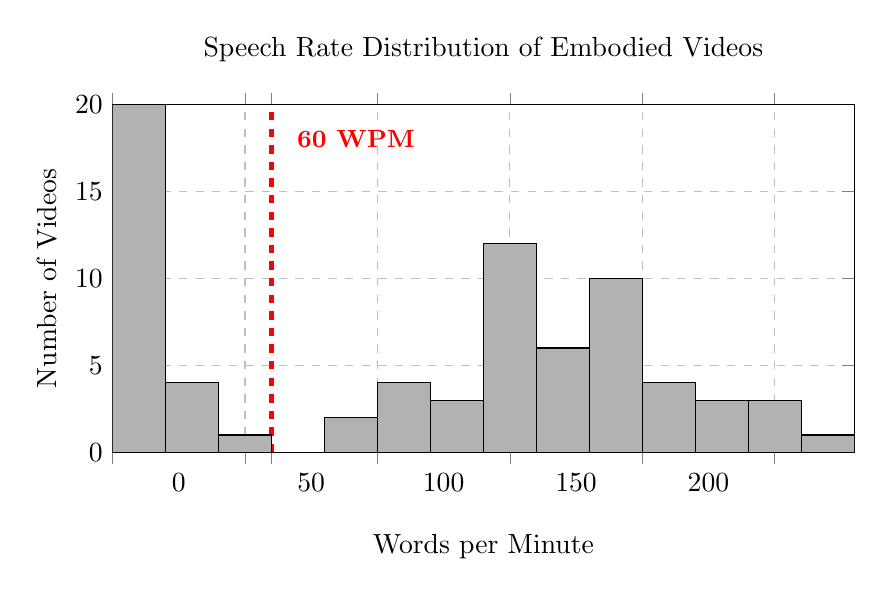
\begin{tikzpicture}
        \begin{axis}[
            ybar interval,
            bar width=0.85,
            width=11cm,
            height=6cm,
            xlabel={Words per Minute},
            ylabel={Number of Videos},
            ymin=0, ymax=20,
            xmin=0, xmax=280,
            xtick={0,50,100,150,200,250},
            ymajorgrids=true,
            grid style=dashed,
            title style={yshift=6pt},
            title={Speech Rate Distribution of Embodied Videos},
            extra x ticks={60},
            extra x tick labels={},
            extra x tick style={grid=major, grid style={red, dashed, line width=1.5pt}},
        ]
            \addplot+[fill=gray!60, draw=black, hist={bins=14, data min=0, data max=280}] table [y index=0] {
                data
                5.6
                248.6
                190.0
                262.0
                166.9
                153.1
                146.5
                164.8
                198.5
                112.9
                206.5
                6.3
                190.9
                185.0
                7.1
                233.1
                149.2
                159.8
                158.9
                25.7
                29.4
                38.2
                183.4
                107.2
                141.0
                14.4
                99.0
                157.4
                190.7
                117.9
                157.9
                196.9
                5.4
                5.5
                159.5
                154.3
                252.1
                8.4
                218.8
                187.7
                105.7
                190.2
                214.5
                8.0
                8.2
                202.6
                25.0
                11.3
                11.4
                172.0
                175.0
                13.3
                96.3
                5.6
                58.3
                9.7
                6.1
                130.6
                251.1
                5.4
                154.8
                9.1
                199.5
                147.0
                16.3
                220.6
                230.7
                136.3
                7.9
                167.2
                138.6
                174.8
                11.8
            };
            \node[red, font=\small\bfseries, anchor=west] at (axis cs:66,18) {60 WPM};
        \end{axis}
    \end{tikzpicture}
    \caption{Speech rate distribution of embodied videos showing a bimodal pattern. The dashed red line indicates the 60~WPM threshold used to distinguish verbally embodied from visually embodied videos. No videos fall between 58.3 and 96.3~WPM.}
    \label{fig:wpm_bimodal}
\end{figure}

The low-WPM cluster ($n = 26$) corresponds to the visually embodied subgroup, in which the instructor performs physical procedures with little or no verbal narration. As anticipated in the study design, the ASR system produced hallucinated or negligible transcripts for these videos, with a mean value of only 96 words, confirming that transcript-based analysis is not applicable to this subgroup. The high-WPM cluster ($n = 48$) corresponds to the verbally embodied subgroup, in which instructors actively describe their physical actions while performing them, with speech rates comparable to conventional videos (174 vs.\ 167~WPM). The same screening applied to the conventional videos showed no bimodal pattern; instead, a tight unimodal distribution (120--231~WPM, $\sigma = 33.7$) was demonstrated, confirming that the silent demonstration style is specific to the embodied category.

To quantify the importance of the designed stratification, we additionally performed a sensitivity analysis in which the two embodied subgroups were aggregated into a single category. In that configuration, the embodied videos appear to consistently underperform the conventional videos on all transcript-based metrics, including correlation score, word count, and transcript density. The apparent deficit is driven entirely by the silent demonstration videos rather than by the embodied modality itself, illustrating the confounding results that an unstratified design would have produced. All comparisons reported below therefore follow the planned design, contrasting conventional videos ($n = 56$) with verbally embodied videos ($n = 48$), which ensures that both groups contain videos with substantive verbal content and enables a meaningful transcript-based comparison.

\subsection{Transcript Verbosity and Density}

With the verbally embodied subgroup isolated, we first compared the basic transcript characteristics of the two groups. Figure~\ref{fig:res_words} presents the average transcript word count and Figure~\ref{fig:res_dens} presents the transcript density.

Conventional videos average 2{,}637 words per video compared to 2{,}267 words for verbally embodied videos (Figure~\ref{fig:res_words}), a modest difference of 370 words. Transcript density is similar, where conventional videos deliver 160 words per minute compared to 163 words per minute for verbally embodied videos (Figure~\ref{fig:res_dens}). These results confirm that when the silent demonstrations are excluded from analysis, verbally embodied instructors produce verbal content at rates comparable to conventional robotics technology demonstration lecturer videos.

\begin{figure}[h!]
    \centering
    \begin{tikzpicture}
        \begin{axis}[
            ybar,
            bar width=25pt,
            width=8cm,
            height=6cm,
            symbolic x coords={Conv, VerbEmb},
            xtick=data,
            xticklabels={Conv, Verb.\ Emb.},
            ylabel={Word Count},
            ymin=0, ymax=3500,
            enlarge x limits=0.5,
            nodes near coords,
            nodes near coords style={font=\bfseries\footnotesize, yshift=15pt},
            title={Average Transcript Word Count},
            ymajorgrids=true,
            grid style=dashed,
        ]
            \addplot+[fill=gray!60, draw=black, error bars/.cd, y dir=both, y explicit, error bar style={line width=1pt}]
            table [x=Label, y=WordMean, y error=WordSEM] {\datatable};
        \end{axis}
    \end{tikzpicture}
    \caption{Average transcript word count. Conventional and verbally embodied videos contain comparable amounts of spoken content.}
    \label{fig:res_words}
\end{figure}

\begin{figure}[h!]
    \centering
    \begin{tikzpicture}
        \begin{axis}[
            ybar,
            bar width=25pt,
            width=8cm,
            height=6cm,
            symbolic x coords={Conv, VerbEmb},
            xtick=data,
            xticklabels={Conv, Verb.\ Emb.},
            ylabel={Words/Min},
            ymin=0, ymax=200,
            enlarge x limits=0.5,
            nodes near coords,
            nodes near coords style={font=\bfseries\footnotesize, yshift=15pt},
            title={Transcript Density (Words/Min)},
            ymajorgrids=true,
            grid style=dashed,
        ]
            \addplot+[fill=gray!60, draw=black, error bars/.cd, y dir=both, y explicit, error bar style={line width=1pt}]
            table [x=Label, y=DensMean, y error=DensSEM] {\datatable};
        \end{axis}
    \end{tikzpicture}
    \caption{Transcript density. Both groups deliver verbal content at nearly identical rates.}
    \label{fig:res_dens}
\end{figure}

\subsection{Topic Coverage}
The number of distinct topics identified per video provides insight into the breadth of instructional content covered in the video. Figure~\ref{fig:res_topics} shows that both groups cover a comparable number of topics, with conventional videos averaging 4.38 topics and verbally embodied videos averaging 4.65 topics. This indicates that when embodied instructors narrate the procedures of robotics learning in the video, they address a similar breadth of instructional themes as conventional lecturers.

\begin{figure}[h!]
    \centering
    \begin{tikzpicture}
        \begin{axis}[
            ybar,
            bar width=25pt,
            width=8cm,
            height=6cm,
            symbolic x coords={Conv, VerbEmb},
            xtick=data,
            xticklabels={Conv, Verb.\ Emb.},
            ylabel={Topic Count},
            ymin=0, ymax=6,
            enlarge x limits=0.5,
            nodes near coords,
            nodes near coords style={font=\bfseries\footnotesize, yshift=15pt, /pgf/number format/fixed, /pgf/number format/precision=2},
            title={Average Topic Count},
            ymajorgrids=true,
            grid style=dashed,
        ]
            \addplot+[fill=gray!60, draw=black, error bars/.cd, y dir=both, y explicit, error bar style={line width=1pt}]
            table [x=Label, y=TopicMean, y error=TopicSEM] {\datatable};
        \end{axis}
    \end{tikzpicture}
    \caption{Average number of identified topics per video. Both groups cover a comparable breadth of instructional sub-topics.}
    \label{fig:res_topics}
\end{figure}

\subsection{User Study Results}

\subsubsection{Correlation Analysis}
The correlation analysis measures how closely student comments align with the video's stated topics. As shown in Figure~\ref{fig:res_corr}, conventional videos yield an average correlation score of 61.2 compared to 51.3 for verbally embodied videos. This remaining gap of 9.9 points is substantially smaller than the 23.5-point gap observed when all embodied videos (including silent demonstrations) were aggregated, representing a 58\% reduction. The narrowed gap suggests that transcript-based correlation is largely comparable between the two groups when verbal content exist. However, if verbal content is not present with the of only silent videos, there is a significant drop of the correlation between video comments and video topics.

\begin{figure}[h!]
    \centering
    \begin{tikzpicture}
        \begin{axis}[
            ybar,
            bar width=25pt,
            width=8cm,
            height=6cm,
            symbolic x coords={Conv, VerbEmb},
            xtick=data,
            xticklabels={Conv, Verb.\ Emb.},
            yticklabel style={/pgf/number format/fixed},
            ylabel={Score (0-100)},
            ymin=0, ymax=80,
            enlarge x limits=0.5,
            nodes near coords,
            nodes near coords style={font=\bfseries\footnotesize, yshift=15pt},
            title={Average Correlation Score},
            ymajorgrids=true,
            grid style=dashed,
        ]
            \addplot+[fill=gray!60, draw=black, error bars/.cd, y dir=both, y explicit, error bar style={line width=1pt}]
            table [x=Label, y=CorrMean, y error=CorrSEM] {\datatable};
        \end{axis}
    \end{tikzpicture}
    \caption{Average correlation score comparing conventional and verbally embodied videos. The two groups show comparable alignment between student comments and instructional topics.}
    \label{fig:res_corr}
\end{figure}

\subsubsection{Engagement Rate}
Engagement rate is measured as the number of student comments per minute of video duration. As shown in Figure~\ref{fig:res_eng}, verbally embodied videos show a slightly higher engagement rate (0.19 comments/min) compared to conventional videos (0.17 comments/min). This suggests that the physical, hands-on nature of embodied content may prompt slightly more viewer interaction relative to the video's length, even when both groups have comparable verbal density.

\begin{figure}[h!]
    \centering
    \begin{tikzpicture}
        \begin{axis}[
            ybar,
            bar width=25pt,
            width=8cm,
            height=6cm,
            symbolic x coords={Conv, VerbEmb},
            xtick=data,
            xticklabels={Conv, Verb.\ Emb.},
            ylabel={Comments/Min},
            ymin=0, ymax=0.3,
            enlarge x limits=0.5,
            nodes near coords,
            nodes near coords style={font=\bfseries\footnotesize, yshift=15pt, /pgf/number format/fixed, /pgf/number format/precision=2},
            title={Engagement Rate (Comments/Min)},
            ymajorgrids=true,
            grid style=dashed,
        ]
            \addplot+[fill=gray!60, draw=black, error bars/.cd, y dir=both, y explicit, error bar style={line width=1pt}]
            table [x=Label, y=EngMean, y error=EngSEM] {\datatable};
        \end{axis}
    \end{tikzpicture}
    \caption{Engagement rate. Verbally embodied videos generate slightly more student comments per minute than conventional videos.}
    \label{fig:res_eng}
\end{figure}

\subsubsection{Correlation Efficiency}
Efficiency is defined as the ratio of high-confidence correlated comments to total comments. As shown in Figure~\ref{fig:res_eff}, the two groups exhibit nearly identical correlation efficiency: conventional videos score 0.47 and verbally embodied videos score 0.46. This indicates that both instructional modalities are equally effective at eliciting topic-relevant student responses when both contain substantive verbal content.

\begin{figure}[h!]
    \centering
    \begin{tikzpicture}
        \begin{axis}[
            ybar,
            bar width=25pt,
            width=8cm,
            height=6cm,
            symbolic x coords={Conv, VerbEmb},
            xtick=data,
            xticklabels={Conv, Verb.\ Emb.},
            ylabel={Efficiency Ratio},
            ymin=0, ymax=0.6,
            enlarge x limits=0.5,
            nodes near coords,
            nodes near coords style={font=\bfseries\footnotesize, yshift=15pt, /pgf/number format/fixed, /pgf/number format/precision=2},
            title={Correlation Efficiency},
            ymajorgrids=true,
            grid style=dashed,
        ]
            \addplot+[fill=gray!60, draw=black, error bars/.cd, y dir=both, y explicit, error bar style={line width=1pt}]
            table [x=Label, y=EffMean, y error=EffSEM] {\datatable};
        \end{axis}
    \end{tikzpicture}
    \caption{Correlation efficiency. Both groups produce comparable proportions of high-confidence correlated comments.}
    \label{fig:res_eff}
\end{figure}

\subsection{Online User Results}
To evaluate whether the trends observed in the student study persist in a broader public context, we analyzed YouTube comments for the same videos.

\subsubsection{YouTube Percent Correlated}
Figure~\ref{fig:yt_corr} shows the percentage of unique YouTube comments correlated to any video topic. Conventional and verbally embodied videos show virtually identical correlation percentages (20.5\% vs.\ 21.1\%), indicating that both instructional formats elicit comparably topic-focused discussions from a general audience.

\begin{figure}[h!]
    \centering
    \begin{tikzpicture}
        \begin{axis}[
            ybar,
            bar width=25pt,
            width=8cm,
            height=6cm,
            symbolic x coords={Conventional, VerbEmb},
            xtick=data,
            xticklabels={Conv, Verb.\ Emb.},
            yticklabel style={/pgf/number format/fixed},
            ylabel={Percent (0-1)},
            ymin=0, ymax=0.35,
            enlarge x limits=0.5,
            nodes near coords,
            nodes near coords style={font=\bfseries\footnotesize, yshift=15pt, /pgf/number format/fixed, /pgf/number format/precision=3},
            title={YouTube Percent Correlated},
            ymajorgrids=true,
            grid style=dashed,
        ]
            \addplot+[fill=gray!60, draw=black, error bars/.cd, y dir=both, y explicit, error bar style={line width=1pt}]
            table [x=Label, y=PctCorrMean, y error=PctCorrSEM] {\ytdatatable};
        \end{axis}
    \end{tikzpicture}
    \caption{Percentage of YouTube comments correlated to at least one topic. Both groups evoke comparably relevant discourse.}
    \label{fig:yt_corr}
\end{figure}

\subsubsection{YouTube Engagement Rate}
The density of comments per minute on YouTube is presented in Figure~\ref{fig:yt_eng}. Verbally embodied videos generate substantially higher engagement (38.2 comments/min) compared to conventional videos (22.8 comments/min). This suggests that narrated hands-on tutorials generate more viewer interaction than lecture-style content in a public audience context.

\begin{figure}[h!]
    \centering
    \begin{tikzpicture}
        \begin{axis}[
            ybar,
            bar width=25pt,
            width=8cm,
            height=6cm,
            symbolic x coords={Conventional, VerbEmb},
            xtick=data,
            xticklabels={Conv, Verb.\ Emb.},
            ylabel={Comments/Min},
            ymin=0, ymax=55,
            enlarge x limits=0.5,
            nodes near coords,
            nodes near coords style={font=\bfseries\footnotesize, yshift=23pt, /pgf/number format/fixed, /pgf/number format/precision=1},
            title={YouTube Engagement Rate},
            ymajorgrids=true,
            grid style=dashed,
        ]
            \addplot+[fill=gray!60, draw=black, error bars/.cd, y dir=both, y explicit, error bar style={line width=1pt}]
            table [x=Label, y=EngMean, y error=EngSEM] {\ytdatatable};
        \end{axis}
    \end{tikzpicture}
    \caption{YouTube engagement rate. Verbally embodied videos drive substantially higher viewer interaction.}
    \label{fig:yt_eng}
\end{figure}

\subsubsection{Top Topic Percentage}
To assess most interested topics of the videos, we measured the percentage of comments discussing the single most popular topic (Figure~\ref{fig:yt_top}). Conventional and verbally embodied videos show nearly identical top topic percentages (16.6\% vs.\ 16.1\%), indicating that audience attention is comparably focused around central themes in both conventional and embodied learning videos.

\begin{figure}[h!]
    \centering
    \begin{tikzpicture}
        \begin{axis}[
            ybar,
            bar width=25pt,
            width=8cm,
            height=6cm,
            symbolic x coords={Conventional, VerbEmb},
            xtick=data,
            xticklabels={Conv, Verb.\ Emb.},
            ylabel={Percent (0-1)},
            ymin=0, ymax=0.25,
            enlarge x limits=0.5,
            nodes near coords,
            nodes near coords style={font=\bfseries\footnotesize, yshift=15pt, /pgf/number format/fixed, /pgf/number format/precision=3},
            title={Top Topic Percent},
            ymajorgrids=true,
            grid style=dashed,
        ]
            \addplot+[fill=gray!60, draw=black, error bars/.cd, y dir=both, y explicit, error bar style={line width=1pt}]
            table [x=Label, y=TopTopicPctMean, y error=TopTopicPctSEM] {\ytdatatable};
        \end{axis}
    \end{tikzpicture}
    \caption{Percentage of comments on the top topic. Both groups show comparably focused audience engagement.}
    \label{fig:yt_top}
\end{figure}

\subsection{Keypoint Analysis}

To investigate whether the remaining correlation gap between conventional and verbally embodied videos reflects differences in instructional structure, we examined the keypoint metrics extracted by the content analysis model. Figure~\ref{fig:kp_count} and Figure~\ref{fig:kp_strength} present the average keypoint count and average keypoint strength score, respectively.

\begin{figure}[h!]
    \centering
    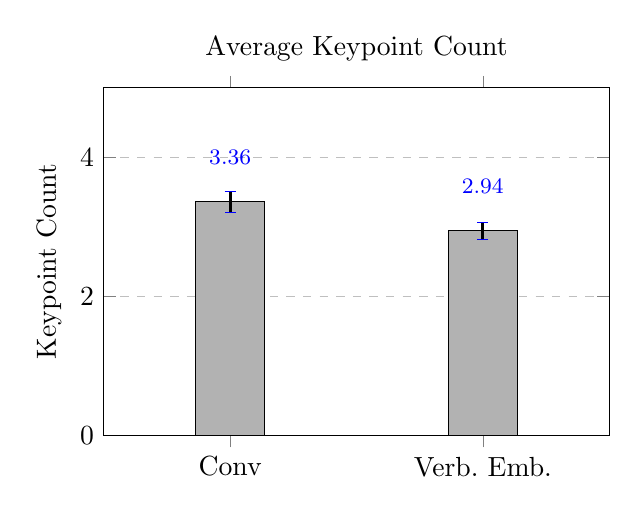
\begin{tikzpicture}
        \begin{axis}[
            ybar,
            bar width=25pt,
            width=8cm,
            height=6cm,
            symbolic x coords={Conv, Verb Emb},
            xtick=data,
            xticklabels={Conv, Verb.\ Emb.},
            ylabel={Keypoint Count},
            ymin=0, ymax=5,
            enlarge x limits=0.5,
            nodes near coords,
            nodes near coords style={font=\bfseries\footnotesize, yshift=10pt, /pgf/number format/fixed, /pgf/number format/precision=2},
            title={Average Keypoint Count},
            ymajorgrids=true,
            grid style=dashed,
        ]
            \addplot+[fill=gray!60, draw=black, error bars/.cd, y dir=both, y explicit, error bar style={line width=1pt}]
            coordinates {
                (Conv, 3.36) +- (0, 0.15)
                (Verb Emb, 2.94) +- (0, 0.12)
            };
        \end{axis}
    \end{tikzpicture}
    \caption{Average number of keypoints identified per video. Verbally embodied videos approach conventional levels in keypoint count.}
    \label{fig:kp_count}
\end{figure}

\begin{figure}[h!]
    \centering
    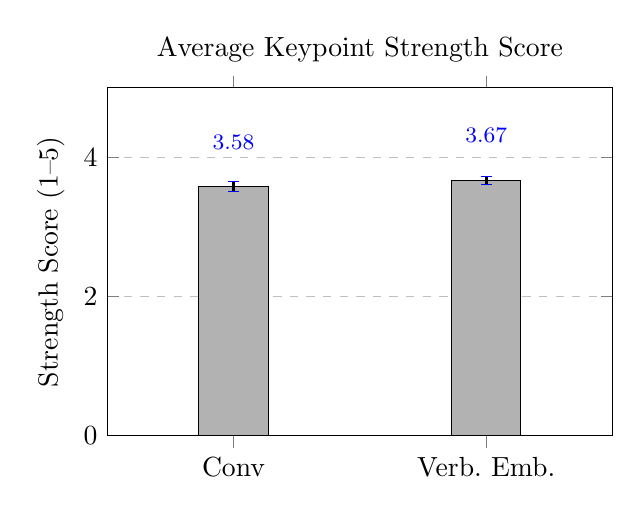
\begin{tikzpicture}
        \begin{axis}[
            ybar,
            bar width=25pt,
            width=8cm,
            height=6cm,
            symbolic x coords={Conv, Verb Emb},
            xtick=data,
            xticklabels={Conv, Verb.\ Emb.},
            ylabel={Strength Score (1--5)},
            ymin=0, ymax=5,
            enlarge x limits=0.5,
            nodes near coords,
            nodes near coords style={font=\bfseries\footnotesize, yshift=10pt, /pgf/number format/fixed, /pgf/number format/precision=2},
            title={Average Keypoint Strength Score},
            ymajorgrids=true,
            grid style=dashed,
        ]
            \addplot+[fill=gray!60, draw=black, error bars/.cd, y dir=both, y explicit, error bar style={line width=1pt}]
            coordinates {
                (Conv, 3.58) +- (0, 0.07)
                (Verb Emb, 3.67) +- (0, 0.06)
            };
        \end{axis}
    \end{tikzpicture}
    \caption{Average keypoint strength score. Verbally embodied videos slightly exceed conventional videos in keypoint reinforcement.}
    \label{fig:kp_strength}
\end{figure}

Conventional videos contain more keypoints on average (3.36 vs.\ 2.94), reflecting the broader topical coverage typical of lecture-style delivery. However, the average keypoint strength---which captures how effectively each keypoint is communicated through repetition and structural reinforcement---is slightly higher for verbally embodied videos (3.67 vs.\ 3.58). This indicates that when embodied instructors narrate, they reinforce their core teaching points at least as effectively as conventional lecturers, despite covering fewer distinct topics.

\subsection{Embodied Phrase Analysis}

The embodied phrase analysis quantifies the frequency and type of physical action language present in each video's transcript. Figure~\ref{fig:phrase_rate} presents the overall embodied phrase rate, and Figure~\ref{fig:cat_breakdown} presents the per-category breakdown.

\begin{figure}[h!]
    \centering
    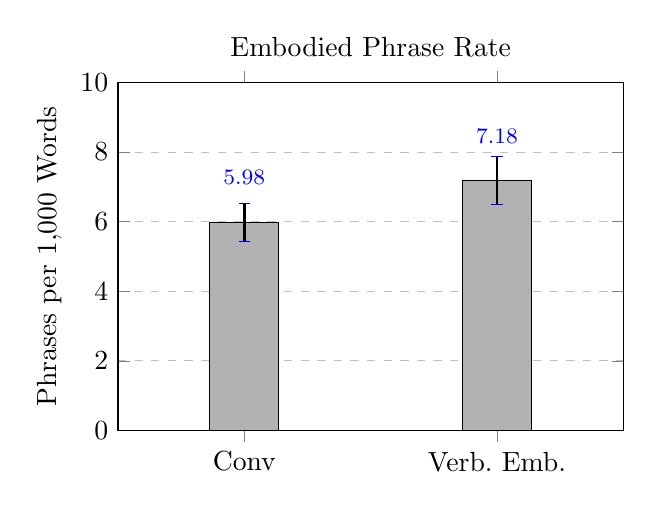
\begin{tikzpicture}
        \begin{axis}[
            ybar,
            bar width=25pt,
            width=8cm,
            height=6cm,
            symbolic x coords={Conv, Verb Emb},
            xtick=data,
            xticklabels={Conv, Verb.\ Emb.},
            ylabel={Phrases per 1{,}000 Words},
            ymin=0, ymax=10,
            enlarge x limits=0.5,
            nodes near coords,
            nodes near coords style={font=\bfseries\footnotesize, yshift=10pt, /pgf/number format/fixed, /pgf/number format/precision=2},
            title={Embodied Phrase Rate},
            ymajorgrids=true,
            grid style=dashed,
        ]
            \addplot+[fill=gray!60, draw=black, error bars/.cd, y dir=both, y explicit, error bar style={line width=1pt}]
            coordinates {
                (Conv, 5.98) +- (0, 0.54)
                (Verb Emb, 7.18) +- (0, 0.69)
            };
        \end{axis}
    \end{tikzpicture}
    \caption{Embodied phrase rate (phrases per 1{,}000 transcript words). Verbally embodied videos contain a higher density of embodied language than conventional videos.}
    \label{fig:phrase_rate}
\end{figure}

\begin{figure}[h!]
    \centering
    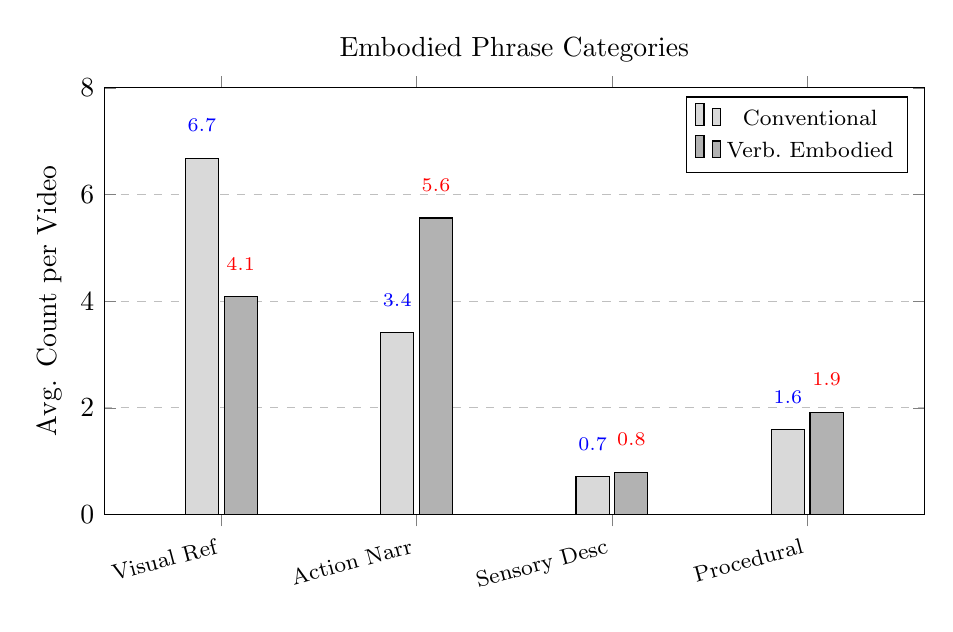
\begin{tikzpicture}
        \begin{axis}[
            ybar,
            bar width=12pt,
            width=12cm,
            height=7cm,
            symbolic x coords={Visual Ref, Action Narr, Sensory Desc, Procedural},
            xtick=data,
            xticklabel style={font=\footnotesize, rotate=15, anchor=north east},
            ylabel={Avg. Count per Video},
            ymin=0, ymax=8,
            enlarge x limits=0.2,
            nodes near coords,
            nodes near coords style={font=\scriptsize, yshift=6pt, /pgf/number format/fixed, /pgf/number format/precision=1},
            title={Embodied Phrase Categories},
            ymajorgrids=true,
            grid style=dashed,
            legend style={at={(0.98,0.98)}, anchor=north east, font=\footnotesize},
        ]
            \addplot+[fill=gray!30, draw=black]
            coordinates {
                (Visual Ref, 6.68)
                (Action Narr, 3.41)
                (Sensory Desc, 0.71)
                (Procedural, 1.59)
            };
            \addplot+[fill=gray!60, draw=black]
            coordinates {
                (Visual Ref, 4.08)
                (Action Narr, 5.56)
                (Sensory Desc, 0.79)
                (Procedural, 1.92)
            };
            \legend{Conventional, Verb.\ Embodied}
        \end{axis}
    \end{tikzpicture}
    \caption{Average count of embodied phrases per video, broken down by category. Conventional videos lead in visual references, while verbally embodied videos lead in action narration.}
    \label{fig:cat_breakdown}
\end{figure}

The embodied phrase rate is 20\% higher in verbally embodied videos than conventional videos (7.18 vs.\ 5.98 phrases per 1{,}000 words), indicating that the narrated embodied tutorials are denser in physical action language. This thus suggests that conventional videos use substantially more visual reference phrases (6.68 vs.\ 4.08 per video). The examples of the visual reference phrases refer to the expressions such as ``look at this'' or ``as you can see'' to capture the on-screen slides or diagrams. In contrast, verbally embodied videos use 63\% more action narration phrases (5.56 vs.\ 3.41), which describe physical manipulation in progress with phrases including ``I'm now connecting this wire to the terminal''. Sensory description and procedural instruction counts are comparable between the two groups.

This pattern suggests that the two modalities employ different verbal strategies. Conventional instructors anchor their language to visual aids, while verbally embodied instructors narrate their physical actions in real time. The higher visual reference count in conventional videos may explain the correlation gap of students comments and video topics between conventional and embodied learning instructional videos. For conventional instructional videos, students watched the slides show in the video and more likely to echo the same terminology in their video comments. Verbally embodied instructors, who focus on describing physical manipulation, producing language that is less likely to be mirrored verbatim in student comments, even when the teaching maybe equally effective.

\subsection{Video Preference Survey Results}
\label{sec:survey_results}

The post-viewing preference survey (Section~\ref{sec:survey_method}) provides a direct, self-reported complement to the comment-based engagement metrics.

\subsubsection{Video Favorability by Modality}
Across the two cohorts, the 65 participants cast 324 favorable and 210 unfavorable video selections over the 20 surveyed videos (8 conventional, 12 embodied). Table~\ref{tab:survey_votes} aggregates the votes by modality. The favorable share, defined as the fraction of all votes for a modality that are favorable, is nearly identical for the two modalities: 61.2\% for conventional videos and 60.3\% for embodied videos. The per-video vote rates are likewise comparable (17.1 vs.\ 15.6 favorable and 10.9 vs.\ 10.2 unfavorable votes per video).

\begin{table}[h!]
    \centering
    \caption{Favorable and unfavorable video selections aggregated by modality.}
    \rowcolors{2}{gray!15}{white}
    \begin{tabular}{l r r}
        \toprule
        & \textbf{Conventional} & \textbf{Embodied} \\
        \midrule
        Videos surveyed & 8 & 12 \\
        Favorable votes & 137 & 187 \\
        Unfavorable votes & 87 & 123 \\
        Favorable votes per video & 17.1 & 15.6 \\
        Unfavorable votes per video & 10.9 & 10.2 \\
        Favorable share & 61.2\% & 60.3\% \\
        \bottomrule
    \end{tabular}
    \label{tab:survey_votes}
\end{table}

Notably, modality does not determine preference at the level of individual videos either: while the three most favored videos were embodied tutorials (36, 32, and 30 favorable votes), the most heavily disfavored videos included both an embodied setup tutorial (22 unfavorable votes) and a conventional question-and-answer recording (20 unfavorable votes). This parity in self-reported preference converges with the near-identical correlation efficiency observed in the comment-based analysis (0.47 vs.\ 0.46), and indicates that learners judge instructional videos primarily by the clarity, applicability, and completeness of the instruction rather than by the presentation modality per se.

\subsubsection{Instructional Feature Preferences}
Table~\ref{tab:survey_features} summarizes the instructional features that participants selected as most useful for their learning.

\begin{table}[h!]
    \centering
    \caption{Instructional features selected as most useful in the post-viewing preference survey. Values are the number (percentage) of respondents selecting each feature; multiple selections were permitted.}
    \rowcolors{2}{gray!15}{white}
    \begin{tabular}{l r r r}
        \toprule
        \textbf{Feature} & \textbf{Cohort 1} & \textbf{Cohort 2} & \textbf{Combined} \\
        & ($n = 51$) & ($n = 14$) & ($n = 65$) \\
        \midrule
        Hands-on experiences & 45 (88.2\%) & 12 (85.7\%) & 57 (87.7\%) \\
        Explanation & 43 (84.3\%) & 12 (85.7\%) & 55 (84.6\%) \\
        Diagrams and charts & 27 (52.9\%) & 8 (57.1\%) & 35 (53.8\%) \\
        Easy-to-follow writing & 24 (47.1\%) & 3 (21.4\%) & 27 (41.5\%) \\
        Body language & 14 (27.5\%) & 4 (28.6\%) & 18 (27.7\%) \\
        Sentiment & 4 (7.8\%) & 4 (28.6\%) & 8 (12.3\%) \\
        Thoroughness$^{\dagger}$ & -- & 11 (78.6\%) & -- \\
        \bottomrule
    \end{tabular}
    \\[2pt]
    {\footnotesize $^{\dagger}$Offered as an option only on the second cohort's form.}
    \label{tab:survey_features}
\end{table}

Two features dominate the participants' self-reported preferences across both cohorts: hands-on experiences (87.7\% of respondents) and clear explanation (84.6\%). The co-dominance of these two features directly mirrors the central finding of the transcript-based analysis: effective embodied instruction couples physical demonstration with active verbal narration, and learners value both channels nearly equally. Notably, body language was selected by only 27.7\% of respondents and sentiment by 12.3\%, indicating that the visible gesturing of the instructor, by itself, is not what learners identify as the useful element of hands-on videos. This asymmetry between highly valued hands-on demonstration and weakly valued body language reinforces the interpretation that the instructional value of embodied videos is carried substantially by the narrated action rather than by visual embodiment alone. In the second cohort, where thoroughness was offered as an option, it was selected by 78.6\% of respondents, suggesting that learners additionally prize complete, uncut demonstrations of procedures.

The free-text justifications were consistent with these quantitative patterns. Participants praised embodied videos for the visibility and traceability of physical procedures (e.g., ``love the wiring in this one, it's very easy to see it piece by piece, and is the least troublesome to recreate yourself''), while the most common criticism of unfavorable videos was the absence of hands-on guidance (e.g., the video ``doesn't provide step-by-step guidance for building or programming robots, making it less useful for hands-on learners'' and is ``too theoretical without direct application''). At the same time, clearly delivered conventional content was also valued (e.g., ``very informative! The video was basically a lecture on its own''), confirming that participants judge videos by the clarity and applicability of the instruction rather than by modality alone.

\subsection{Summary of Findings}

Table~\ref{tab:full_comparison} consolidates all metrics, providing a comprehensive comparison of conventional and verbally embodied videos.

\begin{table}[h!]
    \centering
    \caption{Comprehensive comparison of all metrics between conventional and verbally embodied videos. Values are mean $\pm$ Standard Error of the Mean (SEM).}
    \rowcolors{2}{gray!15}{white}
    \begin{tabular}{l r r}
        \toprule
        \textbf{Metric} & \textbf{Conventional} & \textbf{Verbally Embodied} \\
        & ($n = 56$) & ($n = 48$) \\
        \midrule
        Correlation score ($S_{corr}$) & 61.2 $\pm$ 2.5 & 51.3 $\pm$ 3.6 \\
        Transcript words ($W_{trans}$) & 2{,}637 $\pm$ 355 & 2{,}267 $\pm$ 207 \\
        Transcript density (words/min) & 159.9 $\pm$ 4.4 & 163.1 $\pm$ 5.6 \\
        Speech rate ($R_{wpm}$) & 167 $\pm$ 4.5 & 174 $\pm$ 6.0 \\
        Topic count & 4.38 $\pm$ 0.34 & 4.65 $\pm$ 0.35 \\
        Keypoint count & 3.36 $\pm$ 0.15 & 2.94 $\pm$ 0.12 \\
        Keypoint strength (1--5) & 3.58 $\pm$ 0.07 & 3.67 $\pm$ 0.06 \\
        Embodied phrase count & 12.6 $\pm$ 1.3 & 12.3 $\pm$ 1.0 \\
        Phrase rate (per 1{,}000 words) & 5.98 $\pm$ 0.54 & 7.18 $\pm$ 0.69 \\
        Visual reference & 6.68 $\pm$ 0.79 & 4.08 $\pm$ 0.43 \\
        Action narration & 3.41 $\pm$ 0.43 & 5.56 $\pm$ 0.66 \\
        Sensory description & 0.71 $\pm$ 0.17 & 0.79 $\pm$ 0.18 \\
        Procedural instruction & 1.59 $\pm$ 0.32 & 1.92 $\pm$ 0.34 \\
        Engagement rate (comments/min) & 0.17 $\pm$ 0.03 & 0.19 $\pm$ 0.05 \\
        Correlation efficiency & 0.47 $\pm$ 0.05 & 0.46 $\pm$ 0.05 \\
        YouTube $P_{corr}$ (\%) & 20.5 $\pm$ 2.0 & 21.1 $\pm$ 2.0 \\
        YouTube $E_{yt}$ (comments/min) & 22.8 $\pm$ 5.9 & 38.2 $\pm$ 9.9 \\
        YouTube $P_{top}$ (\%) & 16.6 $\pm$ 1.7 & 16.1 $\pm$ 1.7 \\
        \bottomrule
    \end{tabular}
    \label{tab:full_comparison}
\end{table}

The consolidated results reveal a consistent pattern: verbally embodied videos match or exceed conventional videos on majority of the metric. Verbally embodied instructors speak at equivalent rates, reinforce keypoints more effectively, use more embodied action language per word, and generate higher YouTube engagement. The higher student correlation between conventional and embodied learning instructional videos is likely however associated with the higher frequency of visual reference phrases in conventional videos, which anchor student responses to specific terminology present in the slide presentation rather than reflecting a substantive difference in instructional effectiveness.

%------------------------------------------------

\section{Conclusion}

This study investigated the effectiveness of embodied versus conventional instructional videos for robotics education through transcript-based correlation analysis of student and YouTube comments and demonstrated interesting and unique findings. Recognizing from the outset that the embodied category comprises two fundamentally distinct instructional modalities, including verbally narrated tutorials and silent visual demonstrations, the study was designed around a speech-rate stratification of the embodied videos conducted prior to the comparative analysis. The observed speech rate distribution verified this design, exhibiting a clear bimodal pattern with no videos falling between 58.3 and 96.3 words per minute. Because the silent videos ($n = 26$) produce negligible transcripts by design, making transcript-based analysis inapplicable for those videos, all comparative analyses were conducted between conventional videos ($n = 56$) and verbally embodied videos ($n = 48$), as planned. A complementary sensitivity analysis confirmed the necessity of this design choice: aggregating the silent demonstrations into the embodied category would misleadingly depress all transcript-based metrics, making embodied videos as a whole appear to consistently underperform.

Within this planned three-group design, our results demonstrated that verbally embodied videos are comparable to conventional videos across nearly all transcript-based metrics. Verbally embodied instructors achieved equivalent speech rates (174 vs.\ 167 word per minute), comparable transcript density (163 vs.\ 160 words/min), and similar topic coverage (4.65 vs.\ 4.38 topics). The student correlation gap was modest (61.2 vs.\ 51.3), and the YouTube correlation gap was eliminated entirely (21.1\% vs.\ 20.5\%). Correlation efficiency was virtually identical (0.46 vs.\ 0.47), indicating that both modalities are equally effective at eliciting topic-relevant student responses and engagement.

The keypoint and embodied phrase analyses provided further insight into the instructional characteristics of each modality. Verbally embodied instructors achieved higher keypoint reinforcement scores (3.67 vs.\ 3.58) and 20\% greater embodied phrase density (7.18 vs.\ 5.98 per 1{,}000 words) compared to conventional instructors. The category-level phrase analysis revealed distinct verbal strategies, where the conventional instructional videos rely on visual reference phrases that anchor attention to on-screen materials, while embodied instructors employ action narration to describe physical manipulations in real time.

The post-viewing video preference survey of the 65 study participants corroborated the transcript-based findings through direct self-report. The favorability votes showed near-identical favorable shares for conventional (61.2\%) and embodied (60.3\%) videos, confirming through a third, independent instrument that neither modality is inherently preferred. Hands-on experiences (87.7\%) and clear explanation (84.6\%) were by far the two most frequently selected instructional features, while body language was selected by only 27.7\% of participants. This pattern indicates that learners value the combination of physical demonstration and active verbal narration, rather than visual embodiment alone, converging with the finding that verbally narrated embodied tutorials constitute the most effective instructional format. The free-text justifications echoed this conclusion, with participants criticizing videos lacking step-by-step hands-on guidance while praising both traceable physical procedures and clearly delivered explanations.

Overall, our research results showed that audio and transcript alone can effectively convey embodied instructional content when the instructor actively narrates the physical procedures through the audio content of the video. The effectiveness of this verbal embodied teaching parallels pre-digital video dominated pedagogical teaching tradition where skilled instructors conveyed hands-on knowledge through vivid verbal description without significant visual aids. The bimodal split within embodied videos further suggests that the field of educational video analysis should distinguish between narrated and silent demonstration videos to delivery more powerful instructional design.

Future research will extend our analysis to the visual domain, examining video frames and physical demonstrations directly to capture the instructional content of visually embodied videos which can not be captured by the pure transcript-based analysis. Additionally, the relationship between embodied phrase categories and specific learning outcomes need further investigation with controlled experimental design and analysis.

%------------------------------------------------
\phantomsection
\section*{Declaration of Conflicting Interest} % The \section*{} command stops section numbering

\addcontentsline{toc}{section}{Declaration of Conflicting Interest} % Adds this section to the table of contents

The author(s) declared no potential conflicts of interest with respect to the research, authorship, and/or publication of this article.

\section*{Funding} % The \section*{} command stops section numbering

\addcontentsline{toc}{section}{Funding} % Adds this section to the table of contents

This work was funded by the National Science Foundation, Division of Engineering Education and Centers, Grant/Award Number: 2306285.

%----------------------------------------------------------------------------------------
%	REFERENCE LIST
%----------------------------------------------------------------------------------------
\phantomsection
\bibliography{Bibliography}

%----------------------------------------------------------------------------------------

\end{document}
